\subsection{The NIC-Core Interface}
\label{ssec:niccore-interface}
The \name{}'s NIC Message Reassembler and Packetizer, shown in Figure~\ref{fig:nanoPU}, is responsible for assembling arriving packets into a self-contained RPC message, and then queuing the message into its destination nanotask's FIFO, where the message will remain until that nanotask's thread is scheduled. The message then flows, one word at a time, into the core's head register as the nanotask application processes the words. In the egress direction, the Message Reassembler and Packetizer breaks messages into packets before being sending them to the NIC Datapath.

We make two small modifications to allow the CPU core to interface with this layer of the NIC:
\begin{itemize}
    \item Two former general purpose registers (GPRs) are now reserved for a special purpose: one is the HEAD of the network receive queue, and the other is the TAIL of the network transmit queue. Applications must be compiled to avoid using reserved GPRs for temporary storage. Fortunately, \texttt{gcc} makes it easy to restrict register allocation via command line options.
    \item New control status registers (CSRs) are added for out-of-band communication between the CPU and the NIC. These are used to pass nanotask thread IDs and NIC-driven scheduling information between the NIC and the CPU. 
\end{itemize}

The NIC Message Reassembler and Packetizer hardware maintains transmit and receive FIFOs for each nanotask context (i.e. thread) that is currently pinned to the core. The hardware makes sure that the currently running thread only sees (i.e. reads from and writes to) its own per-context FIFO via the HEAD and TAIL GPRs.

The NIC exposes a {\em message} interface to applications running on the core, instead of a more traditional packet interface.
As a result, the \name{} NIC hardware must be responsible for the termination of the transport layer, including breaking messages into packets, ensuring reliable delivery, and processing message reassembly.

To convey relevant transport information, all messages sent or received by an application carry an 8-byte application header whose format is shown in Figure~\ref{fig:app-headers}. Applications must write the message's destination IP address, destination nanotask context ID and message length at the start of all outgoing messages. (Including the message length allows the NIC to determine when the application has finished writing a complete message.) Similarly, all incoming messages read by any application will begin with the message's source IP address, source nanotask context ID, and message length.

% \begin{figure}
%   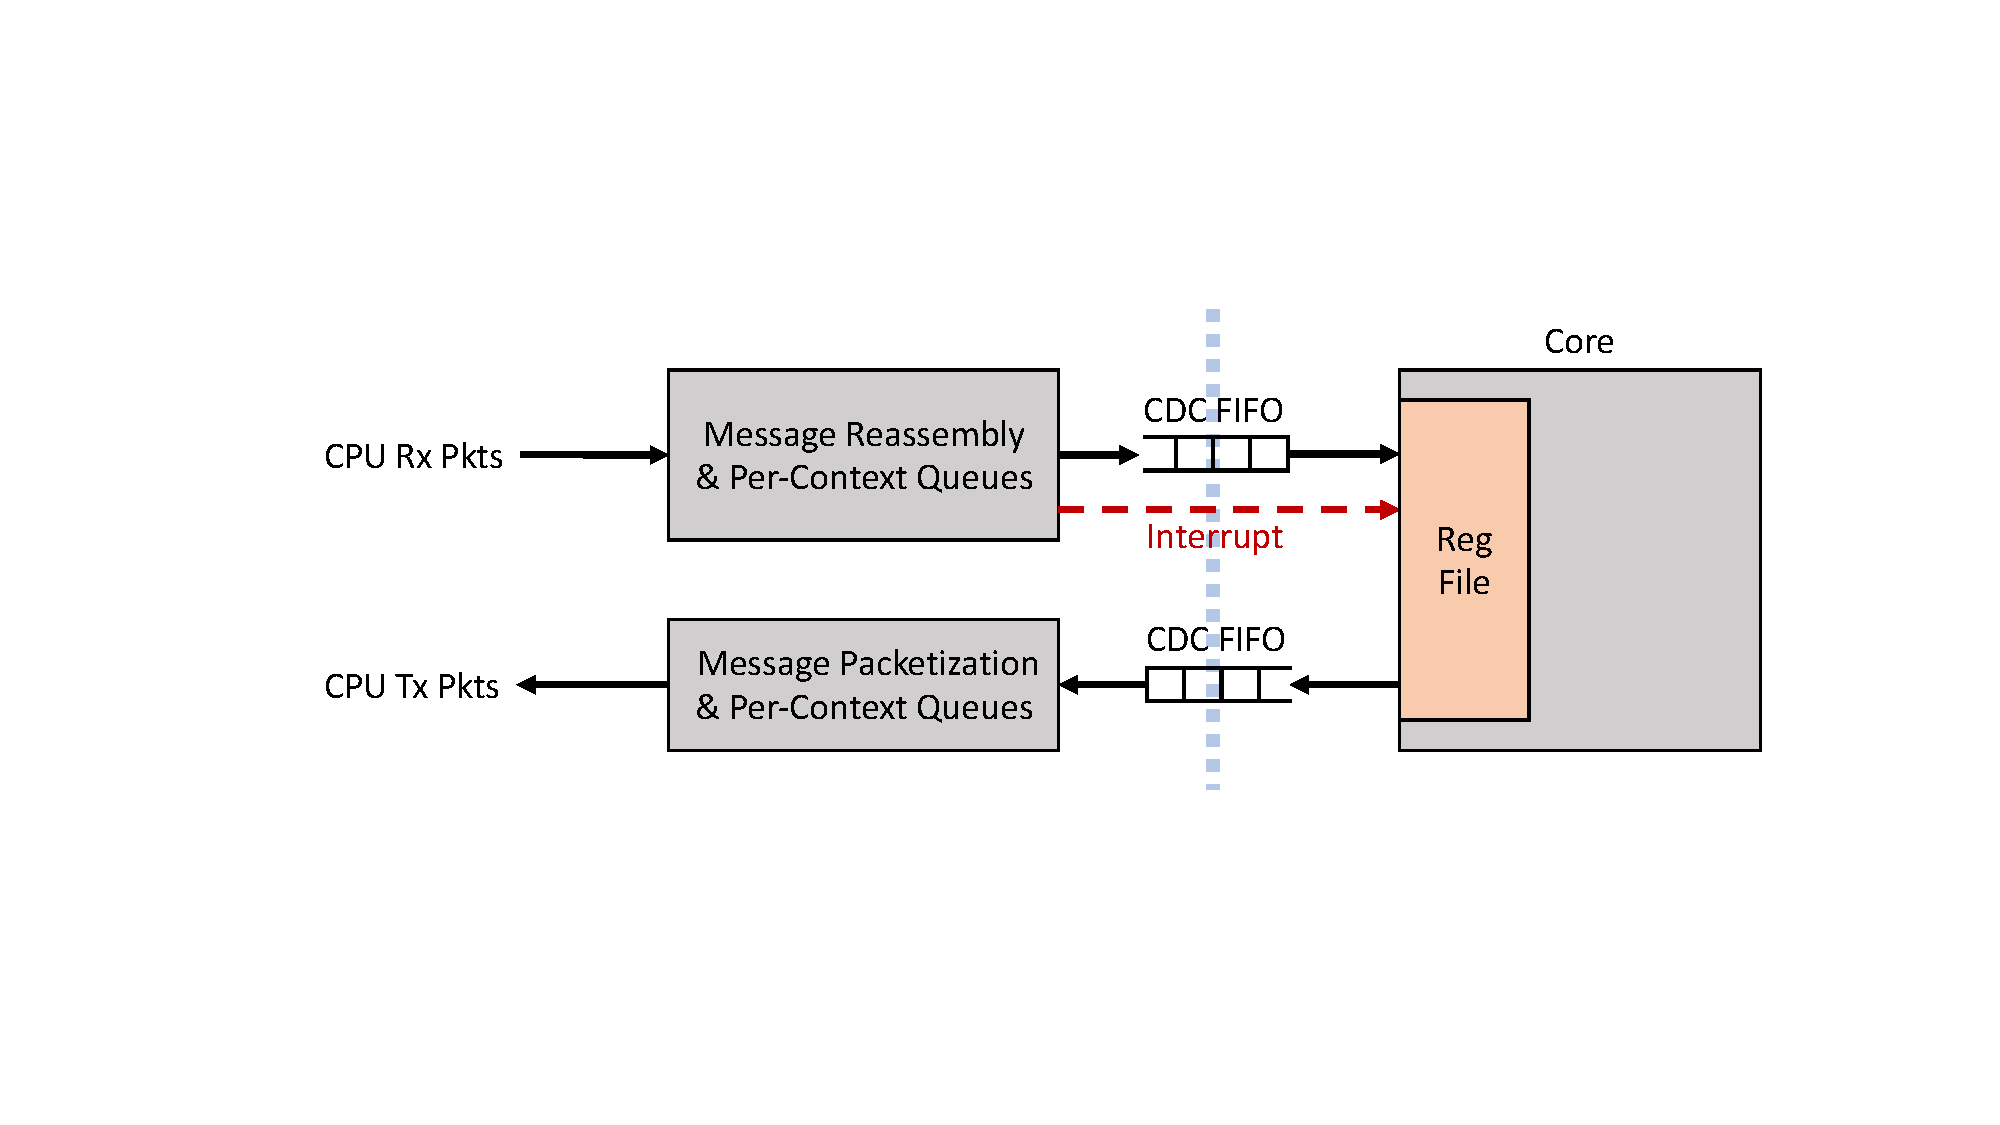
\includegraphics[width=\linewidth]{./figures/NIC-Core-Interface}
%   \caption{Block diagram of the \name{}'s NIC-Core interface.}
%   \label{fig:NIC-Core-Interface}
% \end{figure}

{\lstinputlisting[language=riscv]{code/loopback.S}
\vspace{-20pt}
\captionof{lstlisting}{Loopback with increment: A simple RISC-V \name{} assembly program to register a context \& priority with the NIC, wait for a 16B message to arrive then increment values during loopback from HEAD to TAIL FIFOs..}
\label{lst:asm}}

%\lstinputlisting[caption={Loopback with increment: A simple RISC-V \name{} assembly program to register a context \& priority with the NIC, wait for a 16B message to arrive then increment values during loopback from HEAD to TAIL FIFOs.}, label={lst:asm}]{code/loopback.S}

To illustrate how a \name{} interacts with its NIC, Listing~\ref{lst:asm} shows a simple loopback$+$increment program in RISC-V assembly language.  The program continuously reads 16 byte messages (consisting of two 8 byte integers) from the network, increments the integers, and sends the messages back to their sender. The program is described in more detail below.

The \textbf{\texttt{entry}} procedure registers a nanotask context ID with the NIC using the \texttt{lcurcontext} CSR (in the example, it sets the context ID to be 0). The procedure also sets the priority of the context (again to 0, the most urgent) using the  \texttt{lcurpriority} CSR. It then executes the command by setting the \texttt{lniccmd} CSR to value 1. \texttt{lniccmd} is a bit vector used by supervisor mode software to send commands to the NIC--in this case, it is used to tell the NIC to allocate an RX and a TX queue for context ID$=0$ with priority level$=0$. The \texttt{lniccmd} CSR can also be used to remove context IDs or to update the priority level.\footnote{Although the \texttt{lcurcontext}, \texttt{lcurpriority} and \texttt{lniccmd} CSRs convey hardware commands, they serve a similar purpose to opening or closing a socket in a traditional operating system.}

The \textbf{\texttt{wait\_msg}} procedure waits for a message to arrive in the RX queue by polling the \texttt{lmsgsrdy} CSR until it is set by the NIC, indicating that the context has messages to process. While it is waiting, the application tells the NIC that it is idle by setting the \texttt{lidle} CSR during the polling loop. The NIC thread scheduler uses the idle signal to evict waiting threads and, instead, schedule a new thread with a new message waiting to be processed. 

The \textbf{\texttt{loopback\_plus1\_16B}} procedure simply swaps the source and destination addresses by moving the application header (the first word of every message) from the head register (\texttt{t5}) to the tail register (\texttt{t6}), shown on line 20. It then increments every integer in the received message, appends them to the message being transmitted, and waits for the next message to arrive.

Applications that use variable length messages can use the message length (in the application header) to read the correct number of words from the network RX queue. If an application reads an empty RX queue, the resulting behavior is undefined - similar to reading an uninitialized variable.